\documentclass[journal,12pt,twocolumn]{IEEEtran}

\usepackage{setspace}
\usepackage{gensymb}

\singlespacing


\usepackage[cmex10]{amsmath}

\usepackage{amsthm}

\usepackage{mathrsfs}
\usepackage{txfonts}
\usepackage{stfloats}
\usepackage{bm}
\usepackage{cite}
\usepackage{cases}
\usepackage{subfig}

\usepackage{longtable}
\usepackage{multirow}

\usepackage{enumitem}
\usepackage{mathtools}
\usepackage{steinmetz}
\usepackage{tikz}
\usepackage{circuitikz}
\usepackage{verbatim}
\usepackage{tfrupee}
\usepackage[breaklinks=true]{hyperref}
\usepackage{graphicx}
\usepackage{tkz-euclide}

\usetikzlibrary{calc,math}
\usepackage{listings}
    \usepackage{color}                                            %%
    \usepackage{array}                                            %%
    \usepackage{longtable}                                        %%
    \usepackage{calc}                                             %%
    \usepackage{multirow}                                         %%
    \usepackage{hhline}                                           %%
    \usepackage{ifthen}                                           %%
    \usepackage{lscape}     
\usepackage{multicol}
\usepackage{chngcntr}

\DeclareMathOperator*{\Res}{Res}

\renewcommand\thesection{\arabic{section}}
\renewcommand\thesubsection{\thesection.\arabic{subsection}}
\renewcommand\thesubsubsection{\thesubsection.\arabic{subsubsection}}

\renewcommand\thesectiondis{\arabic{section}}
\renewcommand\thesubsectiondis{\thesectiondis.\arabic{subsection}}
\renewcommand\thesubsubsectiondis{\thesubsectiondis.\arabic{subsubsection}}


\hyphenation{op-tical net-works semi-conduc-tor}
\def\inputGnumericTable{}                                 %%

\lstset{
%language=C,
frame=single, 
breaklines=true,
columns=fullflexible
}
\begin{document}


\newtheorem{theorem}{Theorem}[section]
\newtheorem{problem}{Problem}
\newtheorem{proposition}{Proposition}[section]
\newtheorem{lemma}{Lemma}[section]
\newtheorem{corollary}[theorem]{Corollary}
\newtheorem{example}{Example}[section]
\newtheorem{definition}[problem]{Definition}

\newcommand{\BEQA}{\begin{eqnarray}}
\newcommand{\EEQA}{\end{eqnarray}}
\newcommand{\define}{\stackrel{\triangle}{=}}
\bibliographystyle{IEEEtran}
\providecommand{\mbf}{\mathbf}
\providecommand{\pr}[1]{\ensuremath{\Pr\left(#1\right)}}
\providecommand{\qfunc}[1]{\ensuremath{Q\left(#1\right)}}
\providecommand{\sbrak}[1]{\ensuremath{{}\left[#1\right]}}
\providecommand{\lsbrak}[1]{\ensuremath{{}\left[#1\right.}}
\providecommand{\rsbrak}[1]{\ensuremath{{}\left.#1\right]}}
\providecommand{\brak}[1]{\ensuremath{\left(#1\right)}}
\providecommand{\lbrak}[1]{\ensuremath{\left(#1\right.}}
\providecommand{\rbrak}[1]{\ensuremath{\left.#1\right)}}
\providecommand{\cbrak}[1]{\ensuremath{\left\{#1\right\}}}
\providecommand{\lcbrak}[1]{\ensuremath{\left\{#1\right.}}
\providecommand{\rcbrak}[1]{\ensuremath{\left.#1\right\}}}
\theoremstyle{remark}
\newtheorem{rem}{Remark}
\newcommand{\sgn}{\mathop{\mathrm{sgn}}}
\providecommand{\abs}[1]{\left\vert#1\right\vert}
\providecommand{\res}[1]{\Res\displaylimits_{#1}} 
\providecommand{\norm}[1]{\left\lVert#1\right\rVert}
%\providecommand{\norm}[1]{\lVert#1\rVert}
\providecommand{\mtx}[1]{\mathbf{#1}}
\providecommand{\mean}[1]{E\left[ #1 \right]}
\providecommand{\fourier}{\overset{\mathcal{F}}{ \rightleftharpoons}}
%\providecommand{\hilbert}{\overset{\mathcal{H}}{ \rightleftharpoons}}
\providecommand{\system}{\overset{\mathcal{H}}{ \longleftrightarrow}}
	%\newcommand{\solution}[2]{\textbf{Solution:}{#1}}
\newcommand{\solution}{\noindent \textbf{Solution: }}
\newcommand{\cosec}{\,\text{cosec}\,}
\providecommand{\dec}[2]{\ensuremath{\overset{#1}{\underset{#2}{\gtrless}}}}
\newcommand{\myvec}[1]{\ensuremath{\begin{pmatrix}#1\end{pmatrix}}}
\newcommand{\mydet}[1]{\ensuremath{\begin{vmatrix}#1\end{vmatrix}}}
\numberwithin{equation}{subsection}
\makeatletter
\@addtoreset{figure}{problem}
\makeatother
\let\StandardTheFigure\thefigure
\let\vec\mathbf
\renewcommand{\thefigure}{\theproblem}
\def\putbox#1#2#3{\makebox[0in][l]{\makebox[#1][l]{}\raisebox{\baselineskip}[0in][0in]{\raisebox{#2}[0in][0in]{#3}}}}
     \def\rightbox#1{\makebox[0in][r]{#1}}
     \def\centbox#1{\makebox[0in]{#1}}
     \def\topbox#1{\raisebox{-\baselineskip}[0in][0in]{#1}}
     \def\midbox#1{\raisebox{-0.5\baselineskip}[0in][0in]{#1}}
\vspace{3cm}
\title{EE5609 Matrix Theory}
\author{Kranthi Kumar P}
\date{September 2020}
\maketitle
\newpage
\bigskip
\renewcommand{\thefigure}{\theenumi}
\renewcommand{\thetable}{\theenumi}
Download the python code for ellipse from 
\begin{lstlisting}
https://github.com/kranthiakssy/AI20RESCH14002_PhD_IITH/tree/master/EE5609_Matrix_Theory/Assignment-7
\end{lstlisting}

Download the latex-file codes from 
%
\begin{lstlisting}
https://github.com/kranthiakssy/AI20RESCH14002_PhD_IITH/tree/master/EE5609_Matrix_Theory/Assignment-7
\end{lstlisting}
\section*{Assignment-6\\Coordinate Geometry Exercises}
\subsection*{Problem:}
Conics (1.16):\\
Find points on the curve 
\begin{align}
\vec{x}^T \myvec{\frac{1}{9}&0\\0&\frac{1}{16}}\vec{x}=1
\label{eq:p0}
\end{align}
at which tangents are
\begin{enumerate}[label = (\alph*)]
\item parallel to x-axis
\item parallel to y-axis
\end{enumerate}
\subsection*{Solution:}
The standard ellipse equation can be given by
\begin{align}
\vec{x}^T\vec{D}\vec{x} = 1, \vec{D}=\myvec{\lambda_1&0\\0&\lambda_2},\lambda_1,\lambda_2 >0
\label{eq:s0}
\end{align}
By comparing \eqref{eq:p0} with \eqref{eq:s0}
\begin{align}
\vec{D}=\myvec{\frac{1}{9}&0\\0&\frac{1}{16}}\\
\label{eq:s1}
\lambda_1 = \frac{1}{9}, \lambda_2 = \frac{1}{16}\\
\label{eq:s2}
\vec{V}=\myvec{\frac{1}{9}&0\\0&\frac{1}{16}},\vec{u} = \myvec{0\\0}, f = -1
\end{align}
The Point(s) of contact for ellipse can be given by
\begin{align}
\label{eq:s3}
\vec{q} = \vec{V}^{-1}(k\vec{n}-\vec{u})\\
\label{eq:s4}
k = \pm \sqrt{\frac{\vec{u}^T\vec{V}^{-1}\vec{u}-f}{\vec{n}^T\vec{V}^{-1}\vec{n}}}
\end{align}
\begin{enumerate}[label = (\alph*)]
\item parallel to x-axis\\
The tangents are parallel to x-axis, their direction and normal vectors  are respectively,
\begin{align}
\vec{m}=\myvec{1\\0}, \vec{n}=\myvec{0\\1}
\label{eq:s5}
\end{align}
substituting \eqref{eq:s1}, \eqref{eq:s2} and \eqref{eq:s5} in \eqref{eq:s4}
\begin{align}
k = \pm \sqrt{\frac{1}{\myvec{0&1}\myvec{9&0\\0&16}\myvec{0\\1}}}\\
\implies k = \pm \sqrt{\frac{1}{16}}\\
\label{eq:s6}
\implies k = \pm \frac{1}{4}
\end{align}
substituting \eqref{eq:s6} and \eqref{eq:s2} in \eqref{eq:s3}
\begin{align}
\vec{q} = \myvec{9&0\\0&16}\left(\pm\frac{1}{4}\myvec{0\\1}-\myvec{0\\0}\right)\\
\implies \vec{q} = \myvec{0\\ \pm4}
\end{align}
$\therefore$ the points of contacts with tangents parallel to x-axis are
\begin{align}
\vec{q_{1x}} = \myvec{0\\4}, \vec{q_{2x}} = \myvec{0\\-4}
\end{align} 
\item parallel to y-axis\\
The tangents are parallel to y-axis, their direction and normal vectors  are respectively,
\begin{align}
\vec{m}=\myvec{0\\1}, \vec{n}=\myvec{1\\0}
\label{eq:s7}
\end{align}
substituting \eqref{eq:s1}, \eqref{eq:s2} and \eqref{eq:s7} in \eqref{eq:s4}
\begin{align}
k = \pm \sqrt{\frac{1}{\myvec{1&0}\myvec{9&0\\0&16}\myvec{1\\0}}}\\
\implies k = \pm \sqrt{\frac{1}{9}}\\
\label{eq:s8}
\implies k = \pm \frac{1}{3}
\end{align}
substituting \eqref{eq:s8} and \eqref{eq:s2} in \eqref{eq:s3}
\begin{align}
\vec{q} = \myvec{9&0\\0&16}\left(\pm\frac{1}{3}\myvec{1\\0}-\myvec{0\\0}\right)\\
\implies \vec{q} = \myvec{\pm 3\\ 0}
\end{align}
$\therefore$ the points of contacts with tangents parallel to y-axis are
\begin{align}
\vec{q_{1y}} = \myvec{3\\0}, \vec{q_{2y}} = \myvec{-3\\0}
\end{align}
\end{enumerate}
\begin{figure}[!ht]
	\centering
	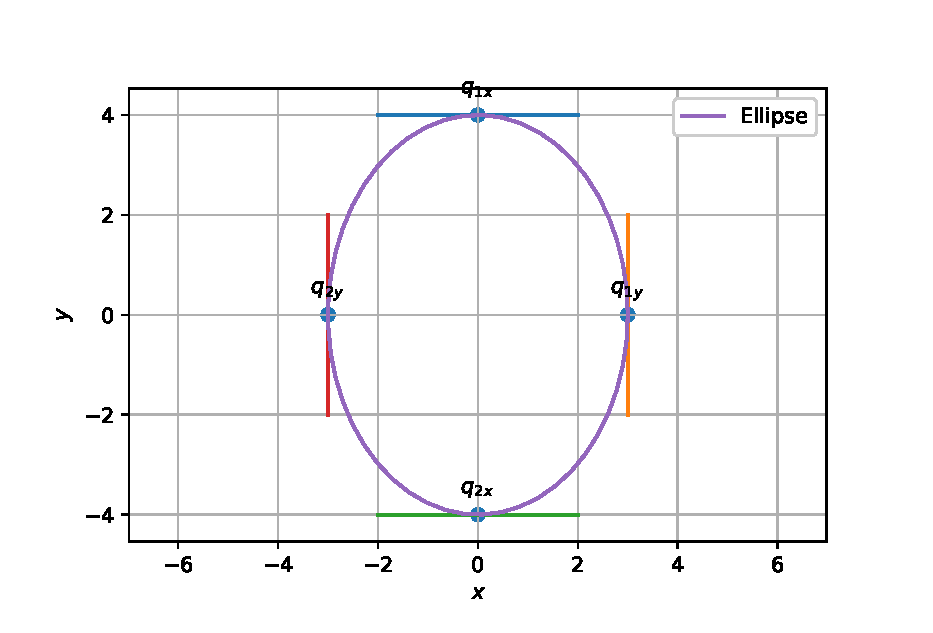
\includegraphics[width=\columnwidth]{ellipse.eps}
	\captionsetup{labelformat=empty}
	\caption{Figure depicting ellipse with tangents}
	\label{myfig}
\end{figure}
\end{document}